\documentclass[UTF8]{mcmthesis}
\mcmsetup{CTeX = FALSE,   % 使用 CTeX 套装时,设置为 true
        tcn = 0000000, problem = A,
        sheet = true, titleinsheet = true, keywordsinsheet = true,
        titlepage = false, abstract = true}
\usepackage{CTEX}
\usepackage{palatino}
\usepackage{lipsum}
\usepackage{graphicx}
\usepackage{listings}
\usepackage{subfigure} 
\usepackage{multirow}
\usepackage{longtable}
\usepackage{graphicx}
\usepackage{caption}
\usepackage{subfigure}
\usepackage{amsmath}
\usepackage{amssymb}
\DeclareMathOperator*{\argmax}{argmax}

 
\usepackage{geometry}
%===============设置正文和数学字体=============================
%有些字体需要安装一些字体文件,注意辨别。
%我参照 MCM论文集的字体 使用如下宏包来定制字体。

\usepackage{graphicx}
\usepackage{subfigure}
%设置段落之间的距离,若不需要删除或者注释掉即可。
\setlength\parskip{.5\baselineskip}
\newtheorem{definition}{Definition}[section]
%\def\abstractname{Summary}%可修改摘要名称

\usepackage{indentfirst}
\setlength{\parindent}{2em}

\usepackage{chngpage}
\usepackage{array}
\usepackage{booktabs} 
\usepackage{threeparttable}
\usepackage{longtable}
\usepackage[numbers,sort&compress]{natbib}
%%% 实现参考文献标号在右上角
\newcommand{\upcite}[1]{\textsuperscript{\textsuperscript{\cite{#1}}}}
%然后引用的时候使用\upcite{}的格式(一般的正常引用格式为\cite{})

\usepackage{titletoc}
\titlecontents{section}[3cm]{\bf \large}{\contentslabel{2.8em}}{}{%
\titlerule*[0.5pc]{$\cdot$}\contentspage}%
\titlecontents{subsection}[4cm]{\normalsize}{\contentslabel{2.5em}}{}{%
\titlerule*[0.5pc]{$\cdot$}\contentspage}%
\titlecontents{subsubsection}[5.3cm]{\normalsize}{\contentslabel{3.0em}}{}{%
\titlerule*[0.5pc]{$\cdot$}\contentspage}%

\title{\large 对现代武器的性价比的评估模型的建立与分析}
\author{}


\date{\today}

\geometry{left=3.0cm,right=3.0cm}

\begin{document}


\begin{abstract}
现今武器在科技支持下飞速发展,各种样式的武器接踵而至,机械巨兽和微小的暗杀机器人也常常作为武器出现在影视屏幕上,那么体积与武器各个部件的体积占比对武器性价比有什么影响,这是一个值得探讨的问题。因此,在理想情况下,我们建立了一套模型,建立武器体积与各项系数与武器性价比的关系,希望能够通过该模型分析在不同情况下,武器的体积发展趋势,对未来武器发展做出一定指导性建议。

\begin{keywords}
武器,体积,性价比; \\ \hspace*{1.2cm}
\end{keywords}
\end{abstract}
\maketitle
%\pagestyle{empty}
\newpage                                                          
\begin{adjustwidth}{-1cm}{0cm}

\setcounter{tocdepth}{3}
\thispagestyle{empty}
\tableofcontents                                                  

\end{adjustwidth}


\newpage

\pagestyle{fancy}

\setcounter{page}{1}
\section{介绍}
\subsection{问题背景}

现代武器在不断的发展中,也有巨大化的趋势,比如从开始的小型舰船到后来可以搭载战斗机的航空母舰,那么在影视资料中常常出现的这种直立式巨型战斗机器是否会成为将来的一种可能武器分支呢,从影片中的资料看,在一些特殊战斗中,这种器械有它自身的优势存在,那么这种优势又能否有足够大的吸引力去催生它的诞生呢,我们难以凭空论断,需要建立分析武器性价比的模型。该模型将不仅能用于这类武器的合理性判定,同时也将对未来武器的发展方向产生指导作用。

\subsection{问题重述}

判断一个武器存在的价值和意义我们认为即判断其性价比。我们需要建立一个模型以通过公式定性评估一个武器的性价比,并由此判断武器大型化是否有价值。


\subsection{问题分析}
武器可以考虑为一个将经费转换为战斗力的机器,故性价比就是武器服役的全程中造成伤害的总量与所需经费的比。造成伤害的总量可以用武器的战斗时长乘以武器的威力描述,经费分为建造经费与后续维护、用于购买资源的经费两部分。我们需要把武器拆分成几个功能模块,并逐个分析。

由于实际问题的复杂性过高,我们需要做出一些基本假设与简化。一些假设是浅显的,一些假设需要佐证,现对于几条假设进行简单陈述以说明其合理性。由于研发成本并不属于某个武器特有,某武器使用的科技也可以移植到其他武器上,该武器也可以完全使用已有的科技,故这里不考虑武器的研发成本,仅考虑建造、维护/驱动成本。后勤补给充足则不用考虑弹药问题,认为在一次战斗中不会消耗完弹药。由于需要考虑的参数较多难以分析求解,我们希望对其中部分参数进行简化。查阅了多种坦克的资料后,基于实际作战中的参数,我们认为装甲厚度与体积的三分之一次幂成正比这一假设是可行的,由此得到的装甲厚度不会对我们武器的性价比造成不利影响。


\section{假设}

\begin{itemize}
\item 不考虑研发成本,成本只包含建造、维护/驱动成本
\item 武器是动力模块、攻击模块、资源模块、管理模块的叠加
\item 武器模块的体积/质量不随着战斗的消耗改变(没有弹药限制)
\item 不考虑武器的外形设计和具体的战斗情景,认为总的战斗力可以通过以上参数评估
\item 除了动力源以外,其它模块均只有一种选择
\item 认为装甲的最佳厚度总是正比于总体积的1/3次幂
\item 武器带来的收益只有战斗价值,不考虑其威慑力等非直接价值
\end{itemize}

\section{符号说明}

\begin{center}
\begin{longtable}{p{.2\textwidth}p{.3\textwidth}m{.4\textwidth}}
\caption{符号说明表}\\
\hline
符号   &单位     & 含义 \\
\hline

$cop$   &无        & 性价比                                  \\
$v_0$   &$m^3$     &总体积\\
$v_1$   &无        & 武器模块体积占比\\
$v_2$   &无        &资源模块体积占比                                                         \\
$v_3$   &无        &动力模块体积占比\\
$\eta$  &W/$m^3$   & 动力源效率 \\                                         
$\rho$  &kg/$m^3$  &总体密度                            \\
$k_1$   &无             &单位武器模块输出\\
$k_2$   &\$/$m^3$          &装甲模块单位价格                                       \\
$k_3$   &\$/$m^3$       &武器模块单位价格                       \\
$k_4$   &\$/$m^3$           &动力源模块单位价格\\
$k_5$   &day(d)        &资源消耗系数\\
$k_6$   &d/kg        &赶赴战场的损失系数\\
$k_7$   &\$/$m^3$       &每次出击单位成本\\
$k_8$   &\$/$m^3$       &每日维护单位成本\\
$k_9$   &d·kg/(W·m)         &机动性增加率\\
$k_{11}$   &         &动力源模块增长系数\\
$\rho_1$   &kg/$m^3$         &装甲密度\\
$\rho_2$   &kg/$m^3$         &装甲外模块密度\\
$mob_0$   &d/m        &机动性阈值\\
$C$   &\$         &控制模块价格\\
$h$   &m         &装甲厚度\\
$t$   &d         &总作战时间\\
$m$   &kg         &总质量\\
$cost_1$   &\$        &建造成本\\
$cost_2$   &\$         &维护成本\\
$mob$   &d/m        &机动性\\
$T$     &d         &单次作战时间\\
\hline
 \end{longtable}
 \end{center}



\section{模型的建立与分析}
\subsection{模型设计思路}
一个武器的实际战斗价值应该在于对于地方军队输出的火力,由于武器的单位体积伤害能力固定,因此武器造成的总伤害应该正比于作战时间$t$和武器体积$v_1v_0$。因此,最终评判武器的目标函数应该正比于$\frac{v_1v_0t}{cost_0}$,即
\begin{equation}
cop=\frac{k_1v_1v_0t}{cost_0}
\end{equation}
\subsubsection{质量的计算}
质量有两方面组成,装甲质量和其余部分质量
\begin{equation}
m=\rho_1hv_0^{\frac{2}{3}}+\rho_2v_0
\end{equation}
这里将h简化为关于正比于$v_0^{\frac{1}{3}}$的函数
\begin{equation}
M=k\rho_1v_0+\rho_2v_0=\rho v_0
\end{equation}
其中$\rho=k\rho_1+\rho_2$
\subsubsection{期望作战天数t的计算}
我们假设武器不会随着战场进化而被淘汰,而只有战斗损坏导致退役。那么,自然地$t$应该受机动性受弹率、机动性和装甲厚度的影响,并且受弹率正比于迎击面积,$v_0^{\frac{2}{3}}$。将比例系数吸收进$mob$的计算
\begin{equation}
t=\frac{h mob}{v_0^{\frac{2}{3}}}
\end{equation}
机动性为了方便计算,使用了拥有x轴截距的线性函数,正比于动力输出,反比于质量
\begin{equation}
mob=k_9\frac{\eta v_3v_0}{m}-mob_0=k_9\frac{\eta v_3}{\rho}-mob_0
\end{equation}
\subsubsection{成本cost的计算}
成本分为两部分,建造成本$cost_1$,维护成本$cost_2$。
\begin{equation}
cost=cost_1+cost_2
\end{equation}

建造成本$cost_1$是武器成本,装甲成本,固定成本(可以认为是通信装置等)以及动力源成本的加和。因为动力效率的增加带来的制造成本增加往往是指数级的,乘上了$e^{k_{11}\eta}$项作为修正,在不需要考虑搭载的动力源效率的时候,可以直接删除这一项,整合进$k_4$中;此外,和上文中同样,装甲的体积已经是$v_0$的函数,直接代入,得
\begin{equation}
cost_1=v_1v_0k_3+v_3v_0k_4\exp(k_{11}\eta)+v_0k_2+C
\end{equation}
$cost_2$分为出击整备成本(弹药、推进剂填充等)和总维护成本.
出击整备成本正比于出击次数$\frac{t}{T}$,资源模块体积$v_2v_0$,因此可以表示为$k_7v_2v_0\frac{t}{T}$,其中单次出击时间T由总的单次续航时间$k_5\frac{v_2v_0}{m}=k_5\frac{v_2}{\rho}$,减去来回奔赴战场/武器启动的时间消耗$k_6$,整合为
\begin{equation}
T=k_5\frac{v_2}{\rho}-k_6
\end{equation}
另一方面,总维护成本正比于作战天数和武器体积,可写为$k_8v_0t$,总成本可写为
\begin{equation}
cost_2=\frac{t}{T}v_2v_0k_7+tv_0k_8
\end{equation}

将全部变量代入cop的表达式中,化简可得
\begin{equation}
cop=k_1v_1\left(t^{-1}(v_1k_3+v_3k_4\exp(k_{11}\eta)+k_2)+\frac{k_7}{\frac{k_5}{\rho}-\frac{k_6}{v_2}}+k_8+\frac{C}{v_0t}\right)^{-1}
\end{equation}

\subsection{模型分析}
\subsubsection{总体积$v_0$}
作为比较有代表意义的量,我们希望$v_0$在这个函数中不会趋向于0或者无穷大。做以下化简
\begin{align*}
&A=\frac{(v_1k_3+v_3k_4\exp(k_{11}\eta)+k_2)}{h mob}\\
&B=\frac{k_7}{\frac{k_5}{\rho}-\frac{k_6}{v_2}}+k_8\\
&D=\frac{C}{mob h}
\end{align*}
则可以将目标函数化简为
\begin{equation}
cop=\frac{k_1v_1}{Av_0^{\frac{2}{3}}+B+Dv_0^{-\frac{1}{3}}}
\end{equation}
使用简单的均值不等式就可以得到$\argmax \limits_{v_0} cop(v_0)=\frac{D}{2A}$
\begin{equation}
V_0=\frac{C}{2(v_1k_3+v_3k_4\exp(k_{11}\eta)+2k_2)}
\end{equation}
可以看到限制$v_0$不宜过大的项为$A$,也即是因为相对于火力增长$\Theta(v_0)$,建造成本增长是$\Theta(v_0^{5/3})$;同时,固定建造成本C的存在则限制了$v_0$不应该太小。整个函数较好地符合了现实里武器体积不应该过大也不过小的情况。

\subsubsection{动力源效率 $\eta$}
同样,我们希望通过对目标函数做$\eta$的偏导,值为0的时候$\eta$的数值不趋于0或者无穷大,将目标函数分母关于$\eta$的部分提出,
\begin{equation}
\frac{k_1v_1}{cop}-\frac{k_7}{\frac{k_5}{\rho}-\frac{k_6}{v_2}}+k_8=\frac{D+EF^{\eta}}{A\eta-B}
\end{equation}
其中
\begin{align*}
&t=A\eta-B\\
&D=\frac{C}{v_0}+v_1k_3+k_2\\
&E=v_3k_4\\
&F=\exp(F)
\end{align*}
需要计算右式的极小值,对$\eta$求偏导等于0得
\begin{align*}
k_{11}EF^{\eta}(A\eta-B-\frac{A}{k_{11}})&=AD
\end{align*}
在$\eta$趋于0时偏导数为负,$\eta$趋于正无穷时为正,因此存在有限极小值点。
在这个函数里,限制$\eta$达不到边界的实际意义在于,过低的动力会导致机动性极低,从而导致战斗天数低,总贡献低;而$\eta$在增大的时候,单位动力源的成本会指数级爆炸增长,将其限制在了一定的范围内。
\subsubsection{对$v_1,v_2,v_3$系数的讨论}
在这部分分析中,认为$v_0$不变,讨论系数$v_1,v_2,v_3$的变化对整个性价比的影响,也就是分析体积分布对最终结果的影响,将对武器研发的组件规划比例做出一定指导。

由上述cop表达式,代入t的表达式,得到
\begin{equation}
cop=k_1v_1\left(\frac{v_0^{\frac{2}{3}}}{h mob}(v_1k_3+v_3k_4\exp(k_{11}\eta)+k_2)+\frac{k_7}{\frac{k_5}{\rho}-\frac{k_6}{v_2}}+k_8+\frac{C}{v_0^{\frac{1}{3}}h mob}\right)^{-1}
\end{equation}

而mob与$v_3$线性相关,再次代入,并进行下面的代换
\begin{align*}
&A=\frac{v_0^{\frac{2}{3}}k_3\rho}{k_9\eta h}\\
&B=\frac{k_2\rho}{k_9\eta h}+\frac{v_0k_4exp(k_{11}\eta)mob_0\rho^2}{k_9^2\eta^2h}+\frac{Cv_0^{-\frac{1}{3}}}{k_9\eta h}\\
&D=\frac{mob_0\rho}{k_9\eta}\\
&E=\frac{k_5}{k_7\rho}\\
&F=\frac{k_6}{k_7\rho}\\
&G=k_8+\frac{v_0^{\frac{2}{3}}k_4exp(k_{11}\eta)\rho}{k_9\eta h}
\end{align*}

得到更简便的关于三个系数的表达式
\begin{equation}
cop=k_1v_1\left(\frac{Av_1+B}{v_3-D}+\frac{1}{E-\frac{F}{v_2}}+G\right)^{-1}
\end{equation}

下面,对该式子进行讨论:可以看到,该式子的主要部分位于分母,分母第一项$\frac{Av_1+B}{v_3-D}$,这一项的现实意义为,当武器体积越大,动力源体积越小,单位服役时间建造成本越大,这是因为,虽然动力会带来成本,但动力源越大,机动性越高,服役时间越长,这会明显体现在平均建造成本中,与之对照的是,在平均建造成本中,武器体积只会带来成本;分母第二项$\frac{1}{E-\frac{F}{v_2}}$,为维修成本除以服役时间的非常数部分,分析可知,平均资源填充成本希望尽可能增加资源体积,因为如果资源体积减小,那么参战次数,或者说往返次数就会增加,奔赴战场消耗的资源这类低效开支就会增加,可见是比较符合实际情况的。

由$v_1+v_2+v_3$=1,结合上述式子,可知,为了保证分母各项都大于零(使其具有现实意义,即成本为正数),则有下面的限制条件
\begin{align*}
&v_3>D\\
&v_2>\frac{F}{E}\\
&v_1>0
\end{align*}

当$v_1$取到上述边界值时,分母作为成本,总是大于G的,所以cop趋于零;当$v_2$取到上述边界值时,分母中第二项趋于正无穷,而分母其他项之和显然也大于G,分子无法趋近于正无穷,所以cop趋于零;当$v_3$取到上述边界值时,而分母第一项$\frac{Av_1+B}{v_3-D}$中的分子部分大于B,所以$\frac{Av_1+B}{v_3-D}$趋于无穷,故而cop趋于零。所以在边界处必定会有cop趋于零,而显然该函数在边界内是连续的,所以存在最优解,也证明了该模型的合理性,对组成部分比例分配有指导意义。

我们查阅了大量数据,通过实际的数据可以大致得到A,B,D,E,F,G的较为合理的取值量级和比例,由数据得到建造成本:维修成本:固定成本$\dot=$75:20:5,武器体积:资源体积:动力装置体积$\dot=$5:2:3,据此得到,A:B:$\frac{1}{E}$:$\frac{1}{F}$:G$\dot=$1:0.16:0.096:4.84:1.58,D$\dot=$0.1。

据此,我们利用matlab作图,得到了下列图像(图中x代表$v_1$,y代表$v_2$,一图中空洞为极值处):
\begin{center} 
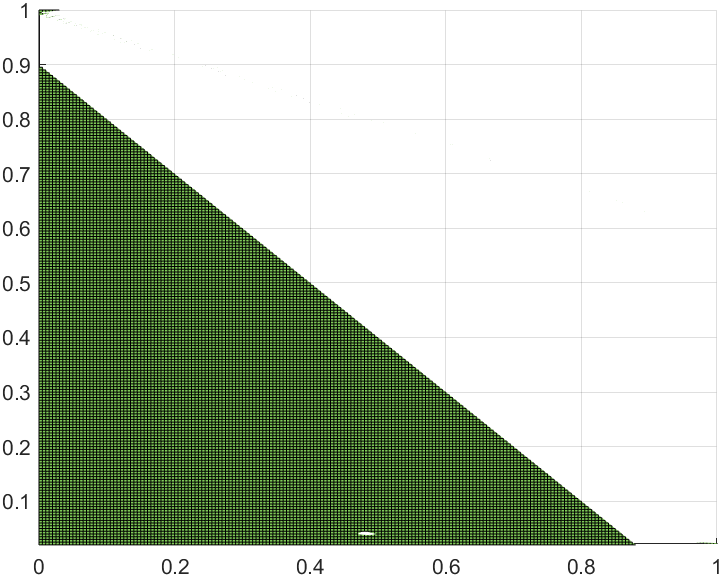
\includegraphics[width=0.8\textwidth]{A2.png} 
\end{center}
\begin{center} 
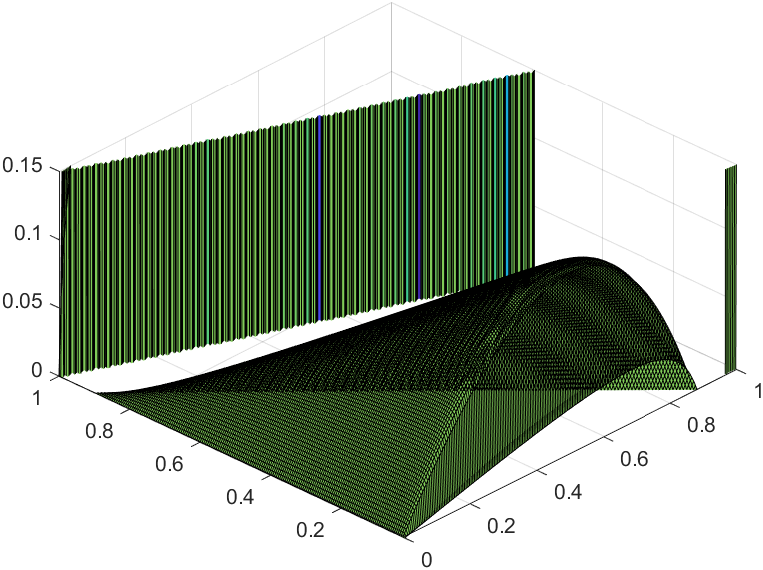
\includegraphics[width=0.8\textwidth]{A1.png} 
\end{center}
由该图可看到,最优解是武器体积占48\%左右,资源体积占3\%左右,也就是说,在现实数据的拟合下得到系数,在理想条件下,该体积分配比较合理,由于模型考虑因素和现实因素有一定差距,同时现实武器不一定是最优解,所以有一定差距是正常的,也意味着模型在有一定合理性的基础下,还需要引入更多因素来评定性价比。

由于上述原因,A,B,D,E,F,G的变化引起的最优解变化更具指导意义,由于直接计算难度过大且繁琐,所以我们利用matlab调整系数,分析变化趋势,挑选比较有代表性的几个变化做些讨论:当A增大时,为了让其变化明显,我们让其按10倍递增,最优解中武器和资源体积因此而不断变小,由(0.48,0.055),变为(0.255,0.03),再变为(0.11,0.025),观察cop表达式,可以看到当分子分母同除$v_1$,可以看到A增大,会让$\frac{1}{v_3-D}$的影响增大,所以动力装置体积有增大趋势显而易见,而A对应现实中的武器成本系数,即武器成本增大时,增加动力装置体积可以增大性价比;当B增大时,最优解中武器和资源体积同样有变小趋势,最优解中武器和资源体积由(0.48,0.055),到(0.455,0.04),再到(0.44,0.03),由cop表达式,也可看出,当A相对较小时,B增大,会导致$v_3$产生增大趋势,而现实中B增大的原因有很多,可能是开始建造武器的固定成本增加,敌人命中率或战场情况改变引起系数C和D的不等比例改变,以及动力成本的增加等等;当D增大时,$v_3-D$影响增大,所以可以判定出$v_3$有变小趋势,matlab作图也说明了这一点,最优解中武器和资源体积由(0.48,0.055),到(0.42,0.05),再到(0.37,0.045),而D是武器躲避伤害所需动力装置体积的最小限制,其增大也就意味着战场情况恶化;当E,F等比减小,也就意味着资源价格上涨,此时资源体积有增大趋势,因为这样可以让运输损耗资源成本占比降低,matlab作图也反映出这一点,最佳资源体积占比由0.055到0.063再到0.105。

\section{模型优缺分析}
\subsection{模型优势}
\begin{itemize}
\item 可解释性强:整个模型的设计逻辑非常清楚,对于武器体积、动力源效率、各功能模块占比接近边界时候的性价比降低都有着与现实相符合的解释。
\item 可优化范围大:在基础的“作战火力/作战成本”框架下,所有部分都可以进行优化。本模型考虑到数学上的可解性,进行了很高程度的简化,采用的函数基本都是线性函数的叠加,并没有考虑边界效应。但这些部分都可以通过修正替换来提升模型参考价值。
\item 可推广性强:在性价比相关的问题上,基本都可以采用“效益/(一次性成本+持续成本)”的模型,例如“汽车评分”,“房屋评分”等。
\end{itemize}

\subsection{模型缺陷}
\begin{itemize}
\item 军械的价值和成本和模型假设相差非常大:在实际中,和平年代的军械设计中,主要成本是研发/技术成本,一般可以占到总成本的50\%以上,尤其在大型军械中可以占到几乎全部;而价值则主要存在于其威慑力,国家形象建设等非直接领域,实际战斗的需求相对较低,而且往往会面临没有完成预计战斗时长就因为性能淘汰,敌方针对等原因提前退役。
\item 模型没有考虑任何的武器具体属性,如结构,运作方式等:在计算价值的时候只是泛泛地将倾泻的弹药数量作为评价标准。而实际上,这些结构的特殊性往往导致军械的评价是量子化而非连续的。
\item 模型没有考虑任何博弈影响:不认为敌人会在遭到武器攻击后调整自己的装备,从而导致模型中参数变化(如杀伤力指标$k_1$),也即是模型为静态的,没有考虑战斗的发展。
\end{itemize}

\subsection{可优化方向}
\begin{itemize}
\item 在原有的模型结构上增加精度:将各个函数进行非线性化处理,优化结果
\item 优化模型结构:模型中对于效益和成本的考量都非常简单,只包含了当下的信息,而实际上一个长时间发挥作用的物品价值需要长久考虑。所以可以增加下列参数:
\begin{itemize}
\item 可以增加时间相关参数,考虑到通货膨胀、物品的性能下降等实际现象可以对它们进行分别修正。
\item 增加风险因素。一般物品的产出量可能达不到统计学范畴,从而简单地用期望代替可能不妥善。在这种情况下,需要先对风险情况下最终受益进行评估再做期望。
\item 增加心理学因素。物品的评估并不只因为客观事实,评价者的主观不可忽略。通过量化“对风险的可接受性”“对于长期价值和短期价值的认识”等心理学因素可以更好地进行价值评估。
\end{itemize}
\end{itemize}
\begin{thebibliography}{123456} 
\bibitem{ref1} 姜启源、谢金星、叶俊. 《数学模型》. 高等教育出版社. 
\end{thebibliography}

\end{document}
